\documentclass[11pt,a4paper]{ctexart}
\usepackage[margin=2.2cm]{geometry}
\usepackage{amsmath,amssymb,bm,booktabs,array,longtable,graphicx,float,xcolor,hyperref,caption}
\definecolor{deepblue}{HTML}{315F85}\definecolor{teal}{HTML}{228C7B}\definecolor{warn}{HTML}{B85C38}
\hypersetup{colorlinks=true,linkcolor=deepblue,urlcolor=deepblue}
\graphicspath{{figures/}}
\captionsetup{font=small,labelfont=bf}
\setlength{\parskip}{0.35em}\setlength{\parindent}{2em}
\newcommand{\vect}[1]{\bm{#1}}
\newcommand{\good}[1]{\textcolor{teal}{\textbf{#1}}}
\newcommand{\risk}[1]{\textcolor{warn}{\textbf{#1}}}
\title{\bfseries COMSOL教师驱动的高频变压器逐匝图模型与在线参数辨识\\[4pt]\large EXP-020至EXP-022 详细实验报告}
\author{高频变压器智能建模项目}
\date{2026年9月16日}

\begin{document}
\maketitle
\begin{abstract}
本报告汇总EXP-020至EXP-022，评估“COMSOL逐匝教师--DAB多窗口观测--低维物理反演--edge-centric GNN”路线是否有效。EXP-020完成单几何$8\times8$电容、电感/互感教师矩阵的网格收敛、双路径电容核验和矩阵求解器集成；EXP-021把教师扩展到12个参数化几何；EXP-022进一步验证理想同构和非理想失配条件下的物理与GNN反演。在前向与反演模型同构时，纯物理反演把端口响应误差降至约1.01\%，GNN直接反演为5.86\%，GNN初值未改变最终精度但缩短约16.8\%的优化时间。在加入频变铜阻、对地寄生、探头增益/延迟及噪声的模型失配实验中，纯物理反演仍取得最佳五参数误差（5.15\%），GNN及混合方法未超过物理基线。因此，当前工作已经证明\good{COMSOL教师可信性、模型链路、低维物理参数化和多窗口反演有效}，并证明GNN可用于快速近似；但尚不能声称\risk{GNN提高了最终辨识精度或已达到实机工程应用水平}。
\end{abstract}

\tableofcontents
\newpage

\section{研究问题与结论先行}
本研究不再尝试仅以一个集中参数$C_{ps}$描述高频变压器，而是用8个匝级节点及完整$\vect C$、$\vect L$耦合矩阵保留内部结构。最终目标是在DAB运行期间利用可获得的端口电压、电流，更新少数可辨识的内部耦合方向，再由物理网络恢复端口和内部响应。

\begin{figure}[H]\centering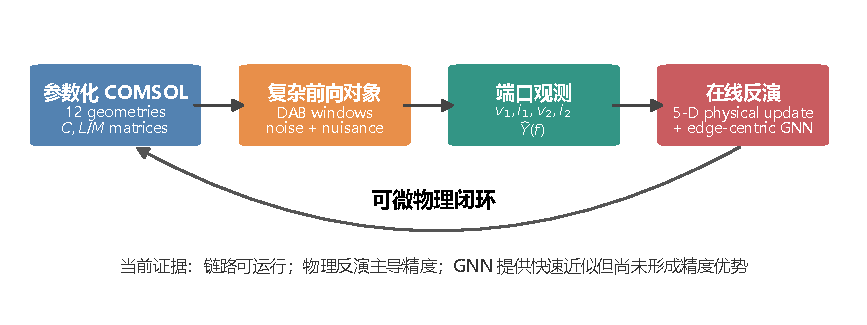
\includegraphics[width=\textwidth]{fig01_workflow.pdf}\caption{当前方法链。COMSOL提供几何相关逐匝矩阵，DAB多窗口提供端口观测，低维物理参数化保证更新后的矩阵合法，GNN作为测量条件化的快速估计器。}\end{figure}

目前可以成立的结论分为三层：
\begin{enumerate}
\item \good{强结论：} 参数化COMSOL教师、矩阵组网、Kron消元、多窗口导纳恢复和低维反演已经形成可运行闭环。
\item \good{中等结论：} GNN从端口频谱和逐匝图中学到了信息，相比完全不更新的标称模型能降低响应误差。
\item \risk{尚不能成立：} GNN优于物理反演、逐条$C_{ij}/M_{ij}$可在线唯一辨识、跨样机泛化以及实机工程精度。
\end{enumerate}

\section{EXP-020：单几何COMSOL逐匝教师的建立与验证}
EXP-020是EXP-021/022的数据基础。它首先回答两个问题：COMSOL能否为每一匝提取满足电路约束的$8\times8$电容和电感/互感矩阵；这些矩阵能否被已有的关联矩阵/Kron求解器直接消费。没有这一步，后续12几何数据集只是一组来源不明的数值。

\subsection{模型结构与物理范围}
模型采用4匝原边、4匝副边的二维轴对称结构。8个铜导体独立编号为P1--P4和S1--S4，外部设置空气域并包含相对磁导率2000的线性磁芯。静电部分把每一匝定义为独立Voltage Terminal；磁场部分逐匝施加电流组合。该模型用于准静态$\vect C$和线性$\vect L/M$教师提取，不包含磁芯非线性、频变复磁导率、集肤/邻近效应和实测接地回路。

\begin{figure}[H]\centering
\begin{minipage}{.48\textwidth}\centering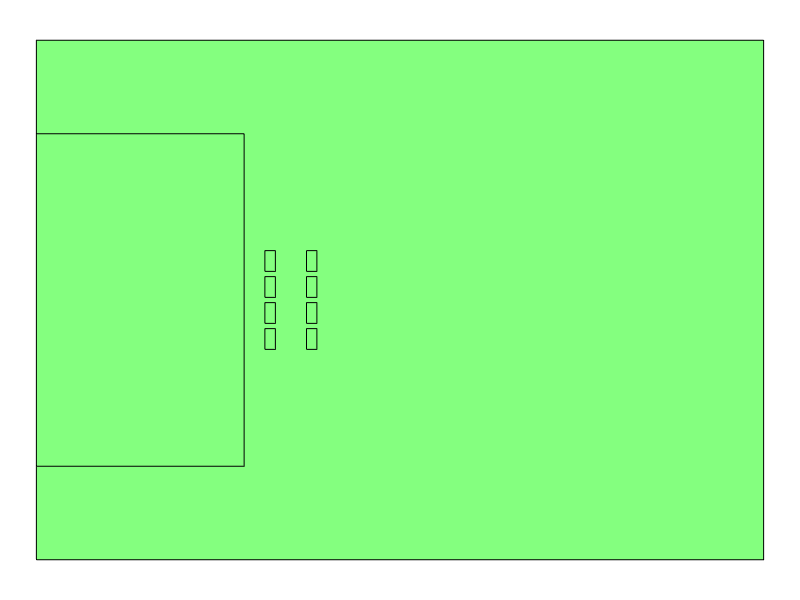
\includegraphics[width=\linewidth]{exp20_geometry.png}\\[-2pt]\small (a) 轴对称几何与8个独立匝导体\end{minipage}\hfill
\begin{minipage}{.48\textwidth}\centering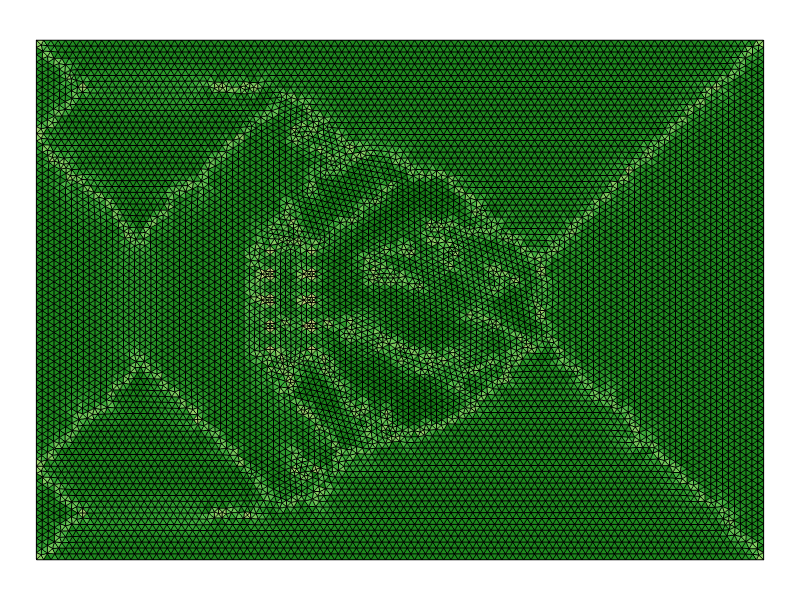
\includegraphics[width=\linewidth]{exp20_final_mesh.png}\\[-2pt]\small (b) 最终细网格（18,898单元）\end{minipage}
\caption{EXP-020 COMSOL基准模型。细网格在绕组、磁芯边界和局部场梯度区域加密，用于最终矩阵验收。}
\end{figure}

\subsection{Maxwell电容矩阵提取}
对第$j$个端子施加1 V，其余7个端子设为0 V，读取所有端子的原生反应电荷$Q_i$，则第$j$次求解直接给出$\vect C$的第$j$列：
\begin{equation}
Q_i=\sum_{j=1}^{8}C_{ij}V_j,\qquad C_{ij}=Q_i\ \text{when}\ V_j=1,\ V_{k\ne j}=0.
\end{equation}
Maxwell矩阵满足$C_{ii}>0$、$C_{ij}<0\ (i\ne j)$。对应的正互电容为$C_{ij}^{mut}=-C_{ij}$，匝对参考导体电容为行和$C_{i0}=\sum_j C_{ij}$。最终最小特征值为$2.125\times10^{-12}$ F，说明约化矩阵正定。

EXP-020还用36个电场能量组合工况独立组装$\vect C$。细网格下，原生Terminal反应电荷法与能量法的Frobenius相对误差为$1.50\times10^{-14}$，最差矩阵元相对误差为$6.45\times10^{-12}$。两种不同提取路径的一致性，是后续将$\vect C$作为监督真值的重要依据。

\subsection{电感/互感矩阵提取}
在线性磁场中，磁能满足
\begin{equation}
W_m=\frac12\vect i^T\vect L\vect i.
\end{equation}
单匝1 A工况给出$L_{ii}=2W_i$；两匝同时1 A时，
\begin{equation}
M_{ij}=W_{ij}-W_i-W_j.
\end{equation}
由8个自感工况和28个两匝组合工况得到完整对称$\vect L/M$。最终最小特征值为$1.303\times10^{-8}$ H，最大非对角耦合系数为0.781。该矩阵只代表准静态线性磁芯教师，不是频变$\vect Z(f)$或交流损耗矩阵。

\begin{figure}[H]\centering
\begin{minipage}{.48\textwidth}\centering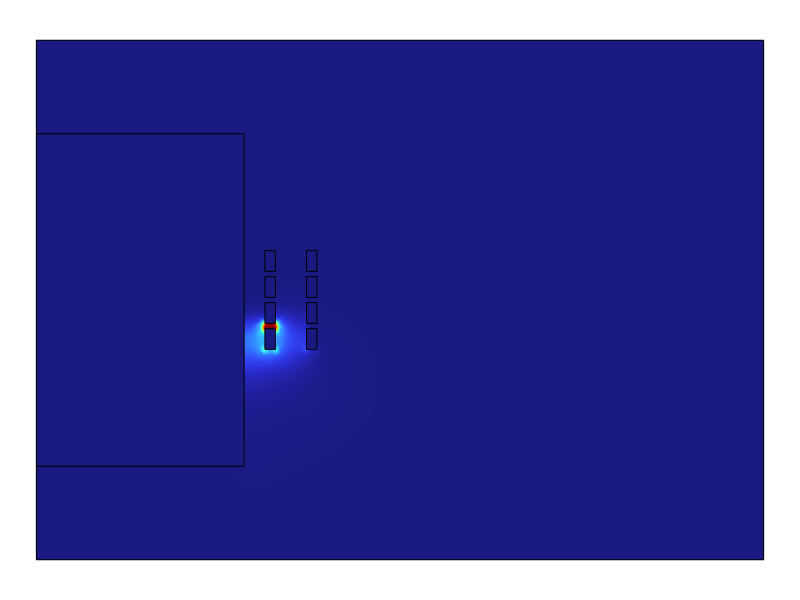
\includegraphics[width=\linewidth]{exp20_electric_field.png}\\[-2pt]\small (a) P1端子激励的电场分布\end{minipage}\hfill
\begin{minipage}{.48\textwidth}\centering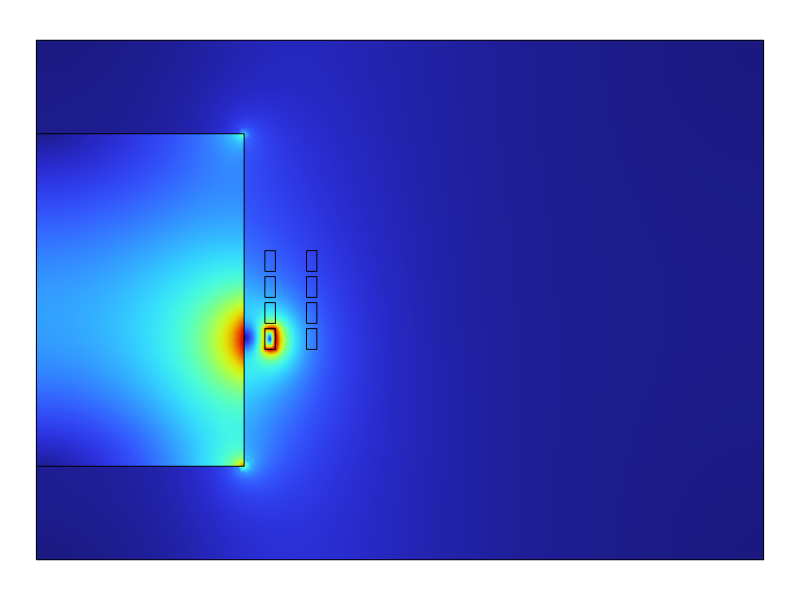
\includegraphics[width=\linewidth]{exp20_magnetic_field.png}\\[-2pt]\small (b) P1电流激励的磁通密度分布\end{minipage}
\caption{EXP-020代表性场结果。电场耦合更局部并受邻近导体屏蔽；磁场通过磁芯形成明显非局部共享磁通。}
\end{figure}

\begin{figure}[H]\centering
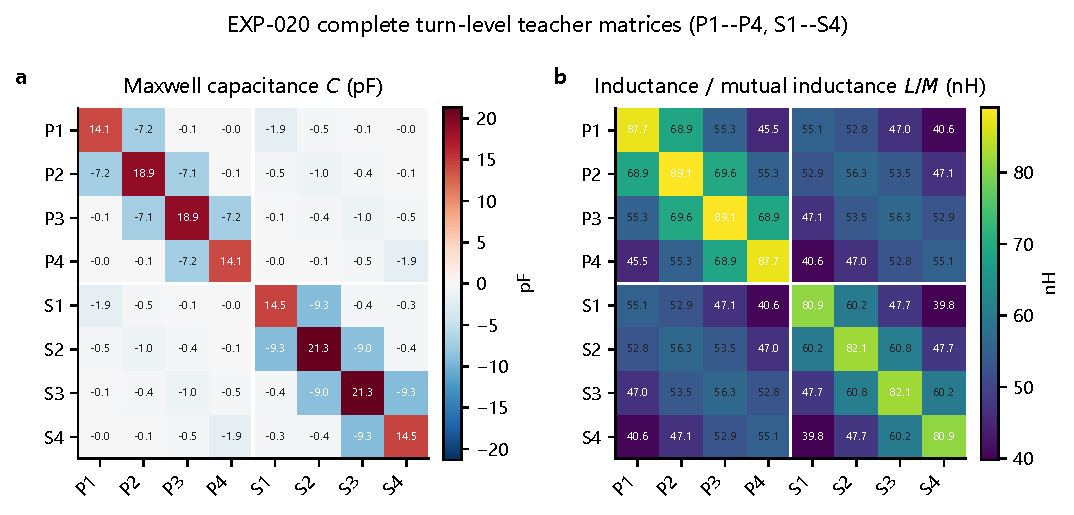
\includegraphics[width=\textwidth]{fig09_exp20_matrix_heatmaps.pdf}
\caption{EXP-020完整逐匝教师矩阵热力图。左：Maxwell电容矩阵（pF），对角元为正、非对角互项为负，白线分隔原边与副边；右：电感/互感矩阵（nH），远距离匝之间仍存在由共享磁芯磁通造成的显著互感。图中保留全部$8\times8$矩阵元，没有筛选或抽样。}
\end{figure}

热力图进一步说明两类耦合不能采用同一删边规则。电容矩阵中，同层相邻匝和面对面的跨绕组项占主导，而非相邻同层项快速衰减；$L/M$矩阵则明显更稠密，即使几何距离较远，也可能因共享主磁通而保持较高互感。因此，后续GNN应把电容边和磁耦合边分开编码，并以端口及内部响应误差而不是单一距离阈值决定可删除的耦合。

\subsection{网格收敛与求解规模}
粗、中、细网格分别包含1,164、2,175和18,898个单元，对应4,762、8,892和76,282个自由度。中到细网格的最大重要矩阵元变化为：$\vect C$对角元0.402\%、互项0.508\%；$\vect L/M$对角元0.100\%、互项0.127\%，均低于预设1\%验收线。三档模型均正常收敛。

\begin{figure}[H]\centering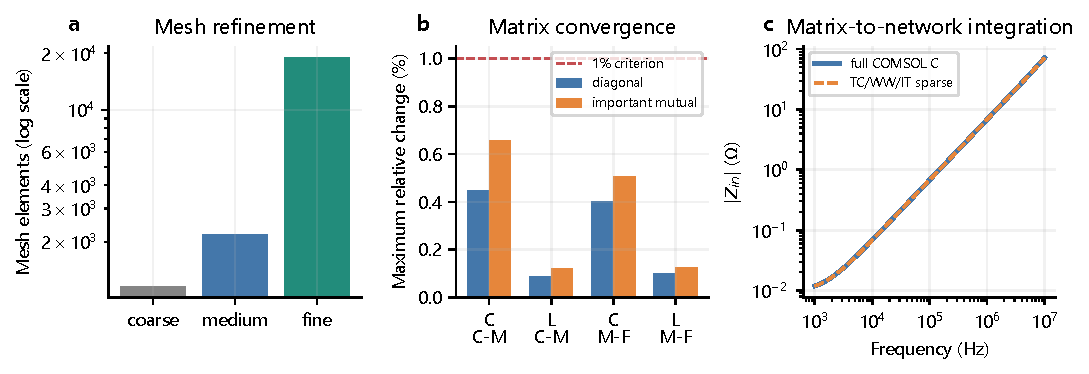
\includegraphics[width=\textwidth]{fig08_exp20_validation.pdf}\caption{EXP-020验证结果。左：三档网格规模；中：$\vect C$和$\vect L/M$的最大相邻网格变化均低于1\%；右：完整COMSOL电容矩阵与文献TC/WW/IT稀疏模型回灌物理网络后的输入阻抗几乎重合。}\end{figure}

\subsection{回灌矩阵求解器与文献稀疏基线}
COMSOL矩阵被映射到
\begin{equation}
\vect Y_n(\omega)=\vect A(\vect R+j\omega\vect L)^{-1}\vect A^T+j\omega\vect C
\end{equation}
并在1 kHz--10 MHz的241个对数频点上求解。内部KCL最大残差为$2.12\times10^{-13}$ A，证明匝序、支路方向和节点映射自洽。

文献TC/WW/IT基线保留全部对参考电容、16条跨绕组边和6条相邻同层匝间边，共22/28条互电容边（78.57\%）。删除的6条非相邻同层边只占总互电容2.054\%。相对完整矩阵，端口导纳Frobenius误差为$1.16\times10^{-7}$，最大幅值差0.00457 dB，内部电压误差$1.09\times10^{-6}$，跨绕组位移电流误差$2.19\times10^{-6}$。

因此，在这个小型、均匀、单层结构中，文献屏蔽规则非常有效；但这不能推广到交错、多层、平面、屏蔽边缘或明显不对称结构。EXP-020也没有在10 MHz范围内发现内部阻抗峰值，不能据此作谐振保持结论。这两个限制正是后续扩大参数化几何和引入学习型边选择的理由。

\section{EXP-021：参数化COMSOL逐匝教师数据}
\subsection{参数化设计}
教师集合采用4匝原边和4匝副边轴对称模型。几何因素为：原副边径向间隙$g_{ps}\in\{1.0,1.5,2.0\}\,$mm、同绕组匝间隙$g_t\in\{0.15,0.25\}\,$mm、副边轴向错位$z_s\in\{0,0.625\}\,$mm，共$3\times2\times2=12$个几何。

每个几何执行8个独立端子电荷工况，按
\begin{equation}
\vect q=\vect C\vect v
\end{equation}
逐列恢复Maxwell电容矩阵。电感/互感矩阵通过36个磁能组合工况求得，并检查互易性$L_{ij}=L_{ji}$。这组数据不再是手工设定的合成矩阵，而是几何和材料驱动的场求解结果。

\begin{figure}[H]\centering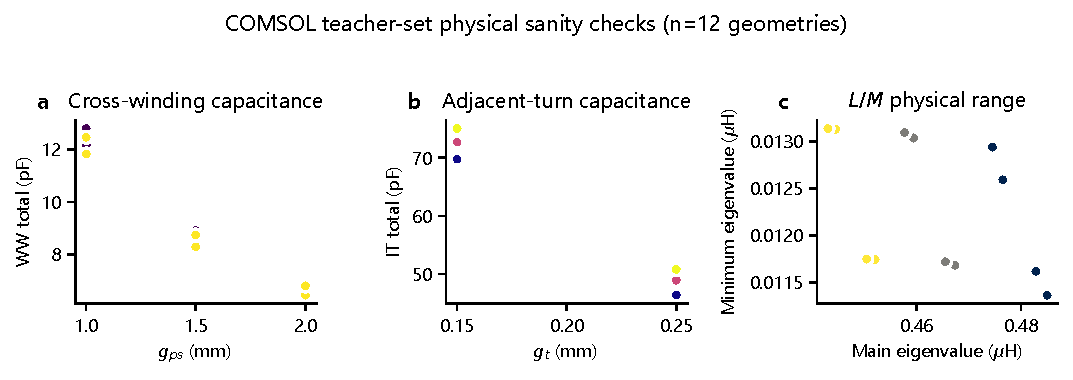
\includegraphics[width=\textwidth]{fig02_teacher_trends.pdf}\caption{12个COMSOL几何的物理趋势检查。跨绕组电容随原副边间隙增加显著下降；相邻匝电容随匝间距增加下降；$\vect L$特征值均保持正值。颜色仅表示另一几何变量，不代表重复测量。}\end{figure}

跨绕组总电容与$g_{ps}$的Pearson相关系数为$-0.977$，相邻匝电容与$g_t$的相关系数为$-0.986$。最大电容矩阵非对称残差为$1.13\times10^{-26}$ F，电感矩阵非对称残差为0。这些结果支持教师数据的数值自洽性，但不等同于网格收敛和实物准确性已经在全部12个几何上得到证明。

\begin{figure}[H]\centering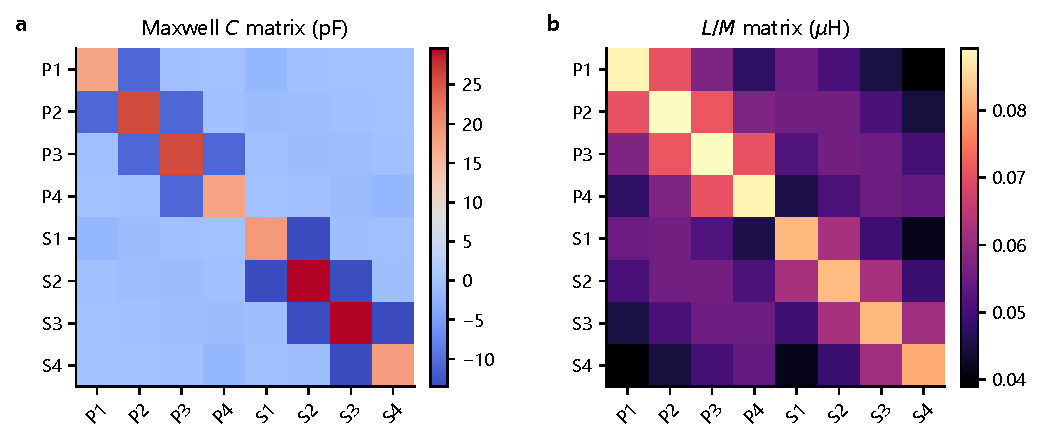
\includegraphics[width=.88\textwidth]{fig03_matrices.pdf}\caption{代表性几何的逐匝矩阵热图。Maxwell电容矩阵对角元为正、互项为负；$L/M$矩阵呈现由共享主磁通产生的稠密非局部耦合。该差异说明电容边和磁耦合边不宜使用同一距离裁剪规则。}\end{figure}

\section{物理网络与五维可辨识参数化}
设8个匝支路的关联矩阵为$\vect A$，节点域导纳为
\begin{equation}
\vect Y_n(\omega)=\vect A(\vect R+j\omega\vect L)^{-1}\vect A^T+\vect G+j\omega\vect C.
\end{equation}
将节点分成端口$p$和内部节点$i$，Kron消元给出
\begin{equation}
\vect Y_p=\vect Y_{pp}-\vect Y_{pi}\vect Y_{ii}^{-1}\vect Y_{ip},\qquad
\vect v_i=-\vect Y_{ii}^{-1}\vect Y_{ip}\vect v_p.
\end{equation}

仅凭少量端口不可能唯一恢复全部矩阵元素，因此在线参数不是64个电容/电感元素，而是
\begin{equation}
\vect\theta=[\theta_{IT},\theta_{WW},\theta_{TC},\theta_m,\theta_\ell]^T.
\end{equation}
前三项分别缩放相邻匝、跨绕组和对参考导体的电容。电容矩阵通过正互电容重新盖章，保持Maxwell结构。对$\vect L_0=\vect U\vect\Lambda\vect U^T$，采用
\begin{equation}
\vect L(\vect\theta)=e^{\theta_m}\lambda_1\vect u_1\vect u_1^T+
e^{\theta_\ell}\sum_{q=2}^{8}\lambda_q\vect u_q\vect u_q^T,
\end{equation}
从而始终保持对称正定。该降维不是为了迎合神经网络，而是由端口可辨识性和物理合法性共同要求。

\section{DAB多窗口观测与GNN结构}
在每个频点使用多个DAB风格相移角和电压比形成不同端口激励方向：
\begin{equation}
\vect I_k=\vect Y_k\vect V_k+\vect N_k,
\qquad
\widehat{\vect Y}_k=\vect I_k\vect V_k^H(\vect V_k\vect V_k^H+\epsilon\vect I)^{-1}.
\end{equation}
多窗口的作用不是简单平均，而是使$\vect V_k$具有足够的数值秩，以分离$\vect Y$的两列。

GNN包含8个匝节点和全候选有向匝对边。节点特征包含位置及原/副边标志；边特征包含相对位置、距离、同绕组/相邻类别及标称$C_{ij},L_{ij}$。三轮edge-centric消息传递后，图表示与复导纳幅相编码融合，输出五个有界对数修正。网络规模为73,925个可训练参数。

训练损失为
\begin{equation}
\mathcal L=\|\widehat{\vect\theta}-\vect\theta\|_2^2+lambda_Y
\|\vect Y_p(\widehat{\vect\theta})-\widehat{\vect Y}_{meas}\|_F^2.
\end{equation}

\section{EXP-021：同构模型下的最小闭环}
数据按几何隔离为8个训练、2个验证和2个测试几何；每个几何60个状态。RTX 5070上训练800 epoch，用时约261 s。

\begin{figure}[H]\centering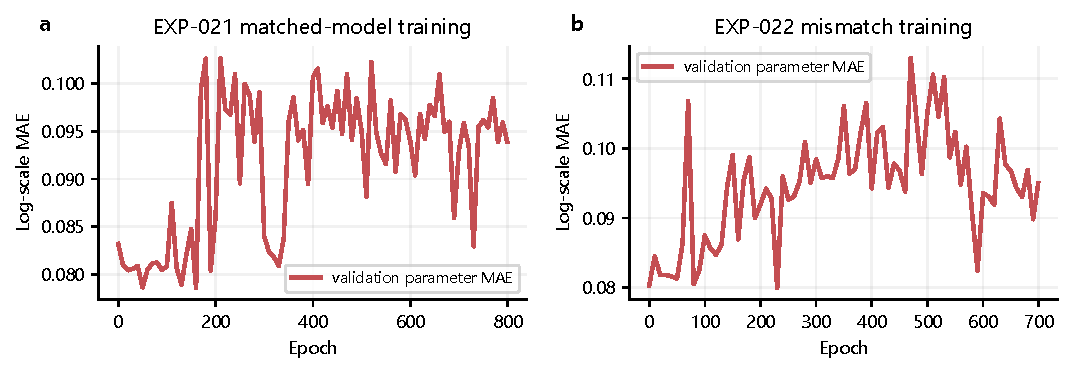
\includegraphics[width=\textwidth]{fig04_training.pdf}\caption{EXP-021与EXP-022的验证参数误差曲线。两项实验均按几何隔离，曲线反映单次随机种子训练，不是置信区间。EXP-022误差平台更高，符合模型失配增加任务难度的预期。}\end{figure}

\begin{table}[H]\centering\caption{EXP-021未见几何测试结果}\begin{tabular}{lccc}\toprule
方法&五参数MAE&端口响应误差&物理优化总耗时\\\midrule
不更新标称矩阵&--&7.603\%&0\\
GNN直接反演&7.569\%&5.864\%&0\\
纯物理反演&\textbf{4.939\%}&1.0081\%&3.816 s\\
GNN初值+物理反演&4.939\%&\textbf{1.0080\%}&3.174 s\\\bottomrule
\end{tabular}\end{table}

GNN相对标称模型使响应误差降低22.87\%，但纯物理反演明显更准确。GNN初值没有改善最终参数精度，只使本轮优化时间减少约16.8\%。这说明网络具有快速近似价值，但在同构小问题上没有必要取代物理求解器。

\begin{figure}[H]\centering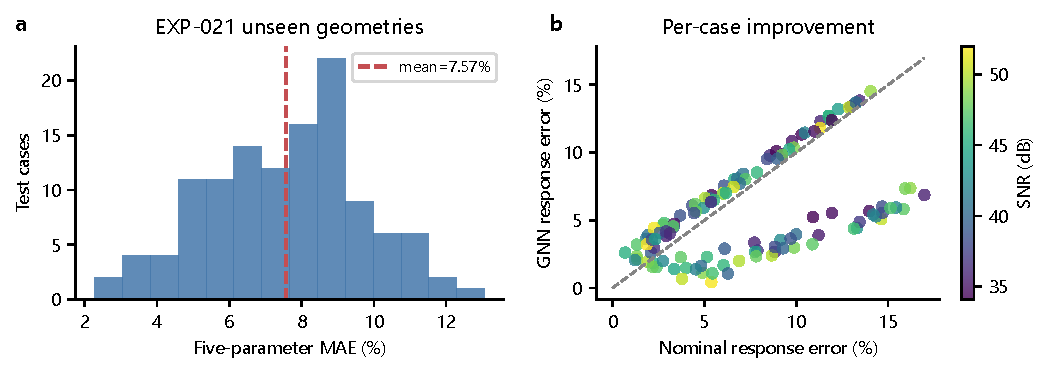
\includegraphics[width=\textwidth]{fig06_test_distribution.pdf}\caption{EXP-021测试样本分布。左：未见几何上五参数MAE；右：每个样本的标称响应误差与GNN响应误差，虚线为等误差线。位于虚线下方表示GNN改善该样本。颜色为观测信噪比。}\end{figure}

\section{EXP-022：前向--反演模型失配}
复杂前向模型进一步加入25--85$^\circ$C温度相关电阻、平方根频变铜阻、原副边0--4 pF非对称对地电容、四测量通道$\pm2\%$增益误差和$\pm45$ ns延迟，以及34--50 dB噪声；反演端对此完全未知。频率范围扩展至20 kHz--1 MHz。每个几何生成80个状态，训练700 epoch，用时约335 s。

\begin{figure}[H]\centering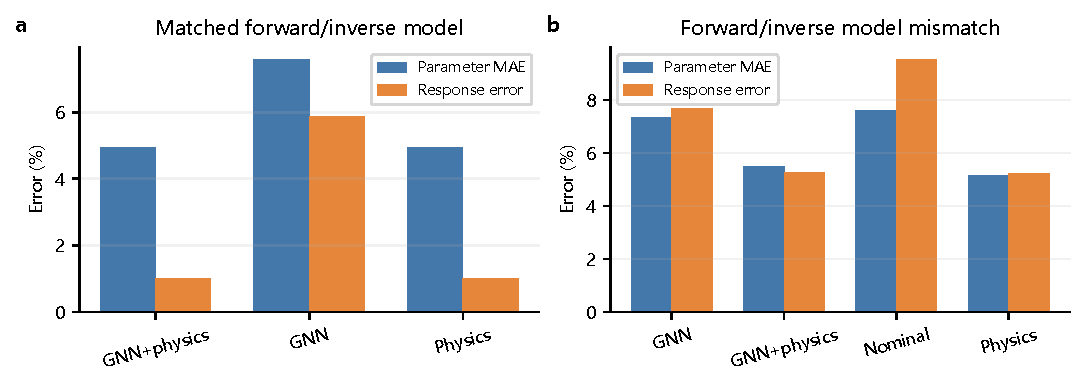
\includegraphics[width=\textwidth]{fig05_method_comparison.pdf}\caption{两项实验的方法比较。左：前向和反演模型同构；右：前向模型包含反演器未知的寄生及测量链路。参数MAE和响应误差具有不同含义：响应拟合良好不保证内部参数正确。}\end{figure}

\begin{table}[H]\centering\caption{EXP-022模型失配测试结果}\begin{tabular}{lcc}\toprule
方法&五参数MAE&简化模型对观测响应误差\\\midrule
标称模型&7.608\%&9.506\%\\
GNN直接反演&7.325\%&7.679\%\\
失配物理反演&\textbf{5.147\%}&\textbf{5.221\%}\\
GNN正则化物理反演&5.478\%&5.242\%\\\bottomrule
\end{tabular}\end{table}

模型失配没有使GNN获得精度优势。探头增益、额外对地电容和真实$\theta_{TC}$可能产生相似端口变化；在没有温度、校准量或额外端口的情况下，这些因素不可被网络凭空区分。该结果反而支持一个重要判断：\risk{继续扩大网络不能替代缺失的观测信息。}

\section{方法是否有效：分项判定}
\begin{figure}[H]\centering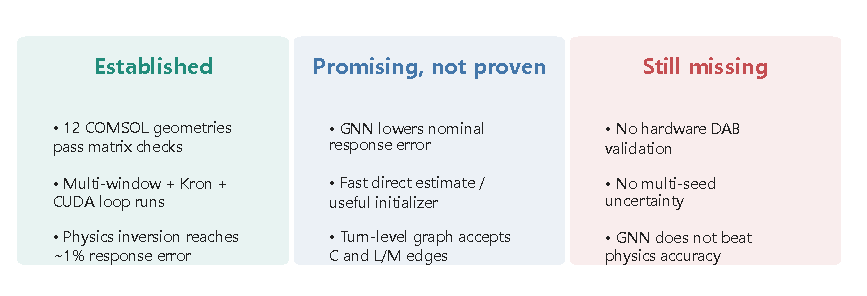
\includegraphics[width=\textwidth]{fig07_evidence_summary.pdf}\caption{当前证据等级。绿色为已经由本轮实验直接支持的结论，蓝色为有趋势但尚需重复和扩展的结论，红色为仍缺少关键证据的部分。}\end{figure}

\begin{longtable}{p{3.0cm}p{2.2cm}p{8.5cm}}\toprule
命题&判定&依据\\\midrule\endhead
COMSOL逐匝矩阵可用于教师&初步成立&12个几何的矩阵结构和几何趋势合理，但只对基准模型做过更高网格验证。\\
多窗口两端口恢复有效&成立（仿真）&不同端口激励方向可以恢复两端口矩阵，并支持后续Kron反演。\\
五维物理降阶有效&成立（仿真）&同构模型下响应误差约1\%；失配时仍优于标称与GNN直接预测。\\
GNN具有信息增益&初步成立&直接GNN在两项实验中均优于不更新标称模型，并可提供快速初值。\\
GNN提高最终精度&不成立&两项实验的最终参数精度均未超过纯物理反演。\\
达到工程/论文最终验证&尚未&无实机DAB、跨样机测试、多随机种子置信区间和真实测量链路标定。\\\bottomrule
\end{longtable}

因此，回答“我们的方法是否比较有效”时，最准确的表述是：
\begin{quote}
当前结果已经证明以COMSOL逐匝矩阵为先验、以多窗口端口信息为观测、以物理合法低维参数为在线更新对象的总体路线有效；GNN作为快速估计模块表现出有限增益，但尚未证明比物理反演更准确。
\end{quote}

\section{下一阶段实验建议}
下一实验应设计为“可观测信息消融”，而不是继续换更大的网络。固定同一组模型失配，依次比较：
\begin{enumerate}
\item 仅两端口$\widehat{\vect Y}$；
\item 加入可测温度；
\item 加入探头增益/延迟校准量；
\item 加入对地共模电流或第三端口观测；
\item 同时加入温度、校准和第三端口。
\end{enumerate}
每一层均比较Fisher最小特征值、参数MAE、响应误差和跨几何泛化。如果附加观测显著改善GNN而纯物理仍受模型残差限制，AI才获得清晰的不可替代价值。

并行的工程准备包括：把COMSOL几何扩大到30--50个；对角点做精细网格收敛；至少运行5个随机种子；制作少匝可引出验证样机，先验证端口扫频和若干代表性匝对，而不是测量全部逐匝电压。

\section{复现信息与局限}
\begin{itemize}
\item GPU：NVIDIA GeForce RTX 5070；PyTorch 2.11.0+cu128。
\item EXP-021：800 epoch、60状态/几何、训练约261 s。
\item EXP-022：700 epoch、80状态/几何、训练约335 s。
\item 划分：训练/验证/测试几何数量为8/2/2；同一几何的状态不跨集合。
\item 主要局限：单随机种子；12个几何；轴对称、线性磁芯和准静态教师；非理想项来自合成分布；没有硬件闭环。
\end{itemize}

\section{最终结论}
EXP-020至EXP-022把项目从“手工合成逐匝网络上的算法验证”推进到“经过收敛核验的COMSOL教师及其在线反演验证”。EXP-020证明逐匝矩阵能够从场模型可靠提取并被矩阵求解器消费；EXP-021证明参数化几何数据链可扩展；EXP-022证明多窗口低维反演可运行，同时揭示模型失配下GNN尚未超过物理基线。最可靠的成果不是某个GNN误差数字，而是建立了场模型、图/矩阵模型和运行端口观测之间的闭环，并明确识别出下一瓶颈是观测缺失与参数混淆，而不是GPU算力或网络容量。

现阶段应坚持“物理反演为主、AI为辅”的技术定位。只有在补充温度、测量链路校准或额外共模观测后，AI能够跨几何、跨工况稳定超过物理基线，才适合把GNN提升为论文的核心算法贡献。

\end{document}
